\documentclass[professionalfont, aspectratio=169]{beamer}
\usetheme{Warsaw}
\usefonttheme{serif}
\usepackage{listings}
\usepackage{amsthm}
\usepackage[]{amsmath}
\title{Beamer Template}
\author{TeXstudio Team}
\begin{document}
\begin{frame}[plain]
	\maketitle
\end{frame}
\begin{frame}{Frame Title}
	\begin{figure}[ht!]
		\centering
		
\includegraphics{screenshot001}
		\caption{wwwwwwwwww}
		\label{fig:www}
	\end{figure}
	\begin{figure}
		\centering
		
\includegraphics[width=0.3\linewidth]{screenshot001}
		\caption{}
		\label{fig:screenshot001}
	\end{figure}
	\begin{equation}
		wwwwww
		\label{www}
	\end{equation}
\end{frame}


\begin{frame}
	\begin{equation}\label{key}
		\int_{1}^{2}=\sum_{1}^{2} q
	\end{equation}
\end{frame}
\begin{frame}
	\begin{equation}\label{key}
		i	\int_{1}^{2}=\sum_{1}^{2}
	\end{equation}
\end{frame}
\begin{frame}
	\begin{equation}\label{key}
		\int_{1}^{2}=\sum_{1}^{2}
	\end{equation}
\end{frame}
\begin{frame}
	\begin{equation}\label{key}
		\int_{1}^{2}=\sum_{1}^{2}
	\end{equation}
\end{frame}
\begin{frame}
	\begin{equation}\label{key}
		\int_{1}^{2}=\sum_{1}^{2}
	\end{equation}
\end{frame}
\begin{frame}
	\begin{equation}\label{key}
		\int_{1}^{2}=\sum_{1}^{2}
	\end{equation}
\end{frame}

\begin{frame}
	\begin{figure}
		\begin{center}
			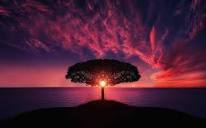
\includegraphics[width=0.3\linewidth]{screenshot002}
		\end{center}
		\caption{wwwwwwwwwwwwwwwwwwwwwwwwwwwwwwwwwww}
		\label{fig:}
	\end{figure}
	It's also possible to override global g:\lstinline{auto_save} value individually per buffer or window. For example, if you have auto save enabled globally, you can opt out some files. And vice versa, opt in some files, when you have auto save disabled globally.
	W  
	\begin{enumerate}
		\end{enumerate}
	\begin{equation}
		\frac{w}{w}	\int_{wwwwww}^{wwww}
		\label{www}
	\end{equation}
	\begin{equation}
		w_w
		\label{wwwwww}
	\end{equation}
	wwwwwwwww
\end{frame}
\end{document}
